\documentclass[10pt]{article}
\usepackage{tikz}
\usetikzlibrary{shapes.misc}
\usepackage[margin=0cm]{geometry}
\pagestyle{empty}
\tikzstyle{every node}=[cross out, draw, red]

\begin{document}

\vspace*{\fill}
\begin{center}
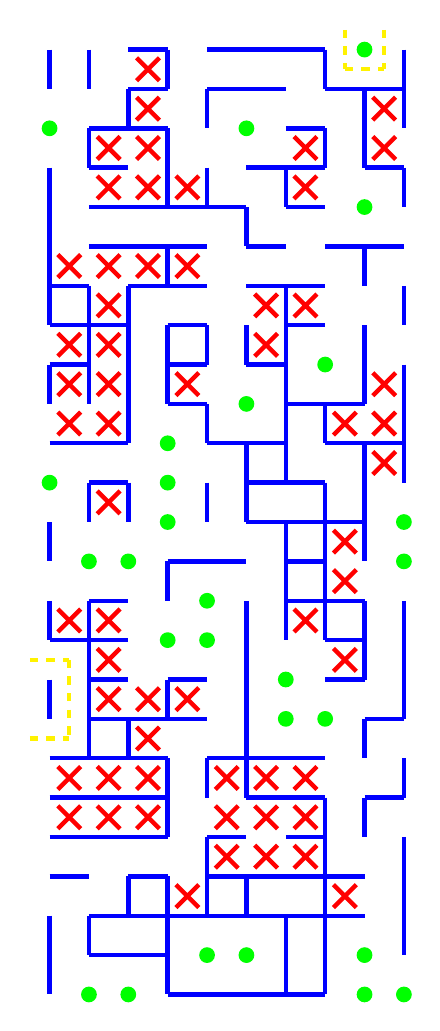
\begin{tikzpicture}[x=0.5cm, y=-0.5cm, ultra thick, blue]
% Walls
    \draw (2,0) -- (3,0);
    \draw (4,0) -- (7,0);
    \draw (2,1) -- (3,1);
    \draw (4,1) -- (6,1);
    \draw (7,1) -- (9,1);
    \draw (1,2) -- (3,2);
    \draw (6,2) -- (7,2);
    \draw (1,3) -- (2,3);
    \draw (5,3) -- (7,3);
    \draw (8,3) -- (9,3);
    \draw (1,4) -- (5,4);
    \draw (6,4) -- (7,4);
    \draw (1,5) -- (4,5);
    \draw (5,5) -- (6,5);
    \draw (7,5) -- (9,5);
    \draw (0,6) -- (1,6);
    \draw (2,6) -- (4,6);
    \draw (5,6) -- (7,6);
    \draw (0,7) -- (2,7);
    \draw (3,7) -- (4,7);
    \draw (6,7) -- (7,7);
    \draw (0,8) -- (1,8);
    \draw (3,8) -- (4,8);
    \draw (5,8) -- (6,8);
    \draw (3,9) -- (4,9);
    \draw (6,9) -- (8,9);
    \draw (0,10) -- (2,10);
    \draw (4,10) -- (6,10);
    \draw (7,10) -- (9,10);
    \draw (1,11) -- (2,11);
    \draw (5,11) -- (7,11);
    \draw (5,12) -- (8,12);
    \draw (3,13) -- (5,13);
    \draw (6,13) -- (7,13);
    \draw (1,14) -- (2,14);
    \draw (6,14) -- (8,14);
    \draw (0,15) -- (2,15);
    \draw (7,15) -- (8,15);
    \draw (1,16) -- (2,16);
    \draw (3,16) -- (4,16);
    \draw (7,16) -- (8,16);
    \draw (1,17) -- (4,17);
    \draw (8,17) -- (9,17);
    \draw (0,18) -- (3,18);
    \draw (4,18) -- (7,18);
    \draw (0,19) -- (3,19);
    \draw (5,19) -- (7,19);
    \draw (8,19) -- (9,19);
    \draw (0,20) -- (3,20);
    \draw (4,20) -- (5,20);
    \draw (6,20) -- (7,20);
    \draw (0,21) -- (1,21);
    \draw (2,21) -- (3,21);
    \draw (4,21) -- (8,21);
    \draw (1,22) -- (8,22);
    \draw (1,23) -- (3,23);
    \draw (3,24) -- (7,24);
    \draw (0,0) -- (0,1);
    \draw (0,3) -- (0,7);
    \draw (0,8) -- (0,9);
    \draw (0,12) -- (0,13);
    \draw (0,14) -- (0,15);
    \draw (0,16) -- (0,17);
    \draw (0,22) -- (0,24);
    \draw (1,0) -- (1,1);
    \draw (1,2) -- (1,3);
    \draw (1,6) -- (1,9);
    \draw (1,11) -- (1,12);
    \draw (1,14) -- (1,18);
    \draw (1,22) -- (1,23);
    \draw (2,1) -- (2,2);
    \draw (2,6) -- (2,10);
    \draw (2,11) -- (2,12);
    \draw (2,17) -- (2,18);
    \draw (2,21) -- (2,22);
    \draw (3,0) -- (3,1);
    \draw (3,2) -- (3,4);
    \draw (3,5) -- (3,6);
    \draw (3,7) -- (3,9);
    \draw (3,13) -- (3,14);
    \draw (3,16) -- (3,17);
    \draw (3,18) -- (3,20);
    \draw (3,21) -- (3,24);
    \draw (4,1) -- (4,2);
    \draw (4,3) -- (4,4);
    \draw (4,7) -- (4,8);
    \draw (4,9) -- (4,10);
    \draw (4,11) -- (4,12);
    \draw (4,18) -- (4,19);
    \draw (4,20) -- (4,22);
    \draw (5,4) -- (5,5);
    \draw (5,7) -- (5,8);
    \draw (5,10) -- (5,12);
    \draw (5,14) -- (5,19);
    \draw (5,21) -- (5,22);
    \draw (6,3) -- (6,4);
    \draw (6,6) -- (6,11);
    \draw (6,12) -- (6,15);
    \draw (6,22) -- (6,24);
    \draw (7,0) -- (7,1);
    \draw (7,2) -- (7,3);
    \draw (7,9) -- (7,10);
    \draw (7,11) -- (7,15);
    \draw (7,19) -- (7,24);
    \draw (8,1) -- (8,3);
    \draw (8,5) -- (8,6);
    \draw (8,7) -- (8,9);
    \draw (8,10) -- (8,13);
    \draw (8,14) -- (8,16);
    \draw (8,17) -- (8,18);
    \draw (8,19) -- (8,20);
    \draw (9,0) -- (9,2);
    \draw (9,3) -- (9,4);
    \draw (9,6) -- (9,7);
    \draw (9,8) -- (9,11);
    \draw (9,14) -- (9,17);
    \draw (9,18) -- (9,19);
    \draw (9,20) -- (9,23);
% Pillars
    \fill[green] (8,0) circle(0.2);
    \fill[green] (0,2) circle(0.2);
    \fill[green] (5,2) circle(0.2);
    \fill[green] (8,4) circle(0.2);
    \fill[green] (7,8) circle(0.2);
    \fill[green] (5,9) circle(0.2);
    \fill[green] (3,10) circle(0.2);
    \fill[green] (0,11) circle(0.2);
    \fill[green] (3,11) circle(0.2);
    \fill[green] (3,12) circle(0.2);
    \fill[green] (9,12) circle(0.2);
    \fill[green] (1,13) circle(0.2);
    \fill[green] (2,13) circle(0.2);
    \fill[green] (9,13) circle(0.2);
    \fill[green] (4,14) circle(0.2);
    \fill[green] (3,15) circle(0.2);
    \fill[green] (4,15) circle(0.2);
    \fill[green] (6,16) circle(0.2);
    \fill[green] (6,17) circle(0.2);
    \fill[green] (7,17) circle(0.2);
    \fill[green] (4,23) circle(0.2);
    \fill[green] (5,23) circle(0.2);
    \fill[green] (8,23) circle(0.2);
    \fill[green] (1,24) circle(0.2);
    \fill[green] (2,24) circle(0.2);
    \fill[green] (8,24) circle(0.2);
    \fill[green] (9,24) circle(0.2);
% Inner points in accessible cul-de-sacs
    \node at (2.5,0.5) {};
    \node at (2.5,1.5) {};
    \node at (8.5,1.5) {};
    \node at (1.5,2.5) {};
    \node at (2.5,2.5) {};
    \node at (6.5,2.5) {};
    \node at (8.5,2.5) {};
    \node at (1.5,3.5) {};
    \node at (2.5,3.5) {};
    \node at (3.5,3.5) {};
    \node at (6.5,3.5) {};
    \node at (0.5,5.5) {};
    \node at (1.5,5.5) {};
    \node at (2.5,5.5) {};
    \node at (3.5,5.5) {};
    \node at (1.5,6.5) {};
    \node at (5.5,6.5) {};
    \node at (6.5,6.5) {};
    \node at (0.5,7.5) {};
    \node at (1.5,7.5) {};
    \node at (5.5,7.5) {};
    \node at (0.5,8.5) {};
    \node at (1.5,8.5) {};
    \node at (3.5,8.5) {};
    \node at (8.5,8.5) {};
    \node at (0.5,9.5) {};
    \node at (1.5,9.5) {};
    \node at (7.5,9.5) {};
    \node at (8.5,9.5) {};
    \node at (8.5,10.5) {};
    \node at (1.5,11.5) {};
    \node at (7.5,12.5) {};
    \node at (7.5,13.5) {};
    \node at (0.5,14.5) {};
    \node at (1.5,14.5) {};
    \node at (6.5,14.5) {};
    \node at (1.5,15.5) {};
    \node at (7.5,15.5) {};
    \node at (1.5,16.5) {};
    \node at (2.5,16.5) {};
    \node at (3.5,16.5) {};
    \node at (2.5,17.5) {};
    \node at (0.5,18.5) {};
    \node at (1.5,18.5) {};
    \node at (2.5,18.5) {};
    \node at (4.5,18.5) {};
    \node at (5.5,18.5) {};
    \node at (6.5,18.5) {};
    \node at (0.5,19.5) {};
    \node at (1.5,19.5) {};
    \node at (2.5,19.5) {};
    \node at (4.5,19.5) {};
    \node at (5.5,19.5) {};
    \node at (6.5,19.5) {};
    \node at (4.5,20.5) {};
    \node at (5.5,20.5) {};
    \node at (6.5,20.5) {};
    \node at (3.5,21.5) {};
    \node at (7.5,21.5) {};
% Entry-exit paths without intersections
    \draw[dashed, yellow] (7.5,0.5) -- (8.5,0.5);
    \draw[dashed, yellow] (-0.5,15.5) -- (0.5,15.5);
    \draw[dashed, yellow] (-0.5,17.5) -- (0.5,17.5);
    \draw[dashed, yellow] (0.5,15.5) -- (0.5,17.5);
    \draw[dashed, yellow] (7.5,-0.5) -- (7.5,0.5);
    \draw[dashed, yellow] (8.5,-0.5) -- (8.5,0.5);
\end{tikzpicture}
\end{center}
\vspace*{\fill}

\end{document}
